\chapter*{Introduction}
\label{introduction.chap.introduction}

Nowadays Image processing is omnipresent in the day to day life of the people. It is present each time we pass by a
CCTV camera, each time we go to the hospital do an IMR, each time we drive our car and pass in front of a speed camera
and each time we use our computer, smartphone or tablet. We just cannot avoid it anymore. The systems using this
technology sometimes are simple, sometimes are complex. Also the usage made of this technology has several different
purposes: space observation, medical, quality of life improvement, surveillance, control, autonomous system, etc.
Henceforth, Image processing is a wide research area and despite having a mass of previous of work already contributed
to, there are still a lot to explore.

Let us take the example of a modern smartphone application which provides facial recognition in order to recognize
people whom are featuring inside a photo. To provide accurate result, this application would have to do a lot of
different processing. Indeed, there are a lot of different cases to handle. We can list (non exhaustively) the weather,
the light exposition, the resolution, the orientation, the number of person, finding the person, distinguishing humans
from animals, etc. All this in order to finally recognizing the person(s) inside the photo. What the application does
not tell you is the complexity of the image processing pipeline behind the scene that can not event be executed in its
entirety on your device. Indeed, image processing is costly in computing ressources and would not meet the time
requirement desired by the user if the entire pipeline was executed on the device. Furthermore, for the final part
"recognize the person on the photo", one needs to feed the pre-processed photo to a neural network trained beforehand
through deep learning techniques in order to give an accurate response. These neural network system usually are
abstracted away in cloud technologies making them available only via Internet. When uploading his image, the user does
not imagine the amount of technologies and computing power that will be used to find who is on the photo.

We now understand that in order to build applications that interact with photos or videos nowadays, we need to be able
to do accurate, fast and scalable image processing on a multitude of devices. In order to achieve this goal, image
processing practitioners needs to have two kinds of tools at their disposal. One will be the prototyping environnement,
a toolbox which allow the practitioner to develop, test and improve its application logic. The other is the production
environnement which deploy the viable version of the application that was developed by the practitioner. Both
environment may not have the same needs. On one hand, the prototyping environment usually requires to have a fast
feedback loop for testing, an availability of state-of-the-art algorithms and existing software so that the practitioner
can easily build upon them and be fast enough so that the practitioner is not waiting for results when testing many
solutions. On the other hand, the production environment must be stable, resilient, fast and scalable.

When looking at standards in the industry nowadays, we notice that Python is the main choice for prototyping. Also,
Python may be enough so that a viable prototype can be pushed in production with minimal changes afterwards. We find it
non-optimal that the practitioner cannot take advantages of many optimisation opportunities, both in term of algorithm
efficiency or better hardware usage, when proceeding this way. It would be much more efficient to have basic low level
building blocks that adapts and fit as mush use cases as possible, so that the practitioner can build upon when
designing its application. Then, if those building blocks can be intelligent enough to take advantage of many
optimization opportunities, the practitioner would have a huge performance improvement, by default, without specifically
tweaking its application.

Finally, it is often known that there is a rule of three about genericity, performance and ease of use. The rule states
that one can only have two of those items by sacrificing the third one. If one wants to be generic and efficient, then
the naive solution will be very complex to use with lot of parameters. If one wants a solution to be generic and easy to
use, then it will be not very efficient by default. If one wants a solution to be easy to use and efficient then it will
not be very generic. This thesis leverages the modern C++ language and its many new features related to genericity and
performance to break this rule in the image processing area. Through continuing work onto the image processing library
Pylene~\cite{carlinet.2018.pylena}, we demonstrate how a library can be generic, efficient and easy to use all at the
same time. This thesis finally attempts, through a static/dynamic bridge, to bring low level tools and concepts from the
static world to the high level and dynamic prototyping world for a better ease of use.

With this philosophy in mind, this manuscript will aim at presenting our thesis work related to the C++ language applied
to the Image Processing domain. It is organized as followed:

\paragraph{Motivation and Context~\ref{part.context_and_Motivations}} presents in-depth specificities about what are the
needs of Image processing. It will then explain who are the different kind of users we find in this area and how this
work may be of interest to them. We will then present the previous work on this subject and what the continuation aims
to be.

\paragraph{Genericity~\ref{part.genericity}} presents a state-of-the-art overview about the notion of genericity. We
will explain its origin, how it has evolved (especially within the C++ language), what issues it is solving, what issues
it is creating. Finally we will tour around existing facilities that allows genericity (intrinsically restricted to
compiled language) to exists in the dynamic world (with interpreted languages such as Python).

\paragraph{Images and Algorithms taxonomy~\ref{part.image_and_algorithms_taxonomy}} presents our first contribution
which is a comprehensive work in the image processing area around the taxonomy of different images families as well of
different algorithms families. This part explains, among others, the notion of concept and how it applies to the
image processing domain.

\paragraph{Images Views~\ref{part.image_views}} presents our second contribution which is a generalization of the
concept of View (from the C++ language) to images. This allows the creation of lightweight, cheap-to-copy images. It
also enable a much simpler way to design image processing pipeline by chaining operations directly in the code in an
intuitive way.

\paragraph{Static dynamic bridge~\ref{part.static_dynamic_bridge}} presents our third contribution which is a way to
grant access to the generic facilities of a compiled language (such as C++) to a dynamic language (such as Python) to
ease the gap between the prototyping phase and the production phase. Indeed, why not enable the practitioner to have
access to production-ready fast algorithm by default? In this part, we discuss some ways of achieving this and offer our
take in the shape of an hybrid solution.

\vspace{1cm}


Image processing has evolved over time to become a field where a very wide array of problematic has arisen. The time
when the 2-dimensional images whose colors were encoded within three 8-bits RGB channels, was a complex construct is
long gone. Instead, and in the last 20 years, there are many new kind of image being brought by the need in new
application domains, be they: medical (3D images from MRI), video games (real time 3D rendering, meshes, visual
effects), astronomy (hyperspectral images with thousands of bands), trees (tree of shapes), graphs (for segmentation,
maps), and so on.

However, despite those kinds of images may originates from different technology domains, they still are being processed
through common, more simple algorithms (such as mathematical morphology) which are the basis of more complex
computations. Thus, it makes sense to have a common base of algorithms to build upon, later, for more complex field
specific applications.

As such, the concept of genericity was introduced. It aims at providing a common ground about how an image should behave
when passed to basic algorithms needed for complex applications. This way, in theory, one only needs to write the
algorithm once for it to work with any given kind of image. In practice, it is also possible to provide a specific
version of a specific algorithm taking advantage of specific properties when available, to for instance, increase
execution speed or decrease memory consumption.

Another aspect that Image processing is in a dire need nowadays is efficiency. Be it with Artificial Intelligence that
needs deep learning on large data set of images or simply the images themselves that are very larges (e.g. 3D mesh with
over 5 million triangles, several hundred of Go for a satellite image), efficiency is pivotal and mandatory. However
genericity and efficiency are often conflicting. Coming up with a solution allying those two aspects is a long time
ongoing work, which is still of topicality nowadays.~\citep{geraud.2012.hdr}

This paper first present in~\ref{part.genericity} our approach of genericity and how we achieve it with efficiency in
mind, through image and algorithm taxonomy. Following, we explain how we can generalize this genericity by introducing a
new tool in~\ref{part.image_views}: the views. They add another abstraction level to images allow one to have a new
approach of writing an image processing pipelines more naturally and without pulling down efficiency with trade-offs.
Finally, we present in~\ref{part.image_and_algorithms_taxonomy} our work on image processing algorithm taxonomy to offer
the user the possibility to have efficient and reusable code by default even when writing prototypes of algorithms.

\vspace{1cm}

As many other numerical fields of computer science, \emph{Computer Vision} and \emph{Image Processing (IP)} have to face
the constantly varying form of the input data. The data are becoming bigger and comes from a wider range of input
devices: the current issue is generally not about acquiring data, but rather about handling and processing it (in a
short time if possible\ldots). In image processing, the two-dimensional RGB model has become too restrictive to handle
the whole variety of \emph{kinds} of image that comes with the variety of images fields. A non-exhaustive list of them
includes: \emph{remote sensing} (satellites may produce hyperspectral images with some thousands of bands),
\emph{medical imaging}, (scans may provide 3D and 3D+t volumes with several modalities), \emph{virtual reality} (RGB-D
cameras used for motion capture provide 2D/3D images with an extra 16-bits \emph{depth} channel), \emph{computational
  photography} (some high-dynamic-range sensors produce 32-bits images to preserve details in all ranges of the
luminance)\ldots

These examples already highlight the need for versatility, but some more domain-oriented applications attempt to broaden
further the definition of images. For example, in digital geometry, one would define images over non-regular domains as
graphs, meshes or hexagonal grids. The increase of image type should not require to write several implementation of the
algorithm. A single version should be able to work on several image types. The~\cref{fig.type.vs.algo2} illustrates this
idea with the same watershed implementation applied on an image 2D, a graph as well as a mesh.

\begin{figure}[htbp]
  \centering
  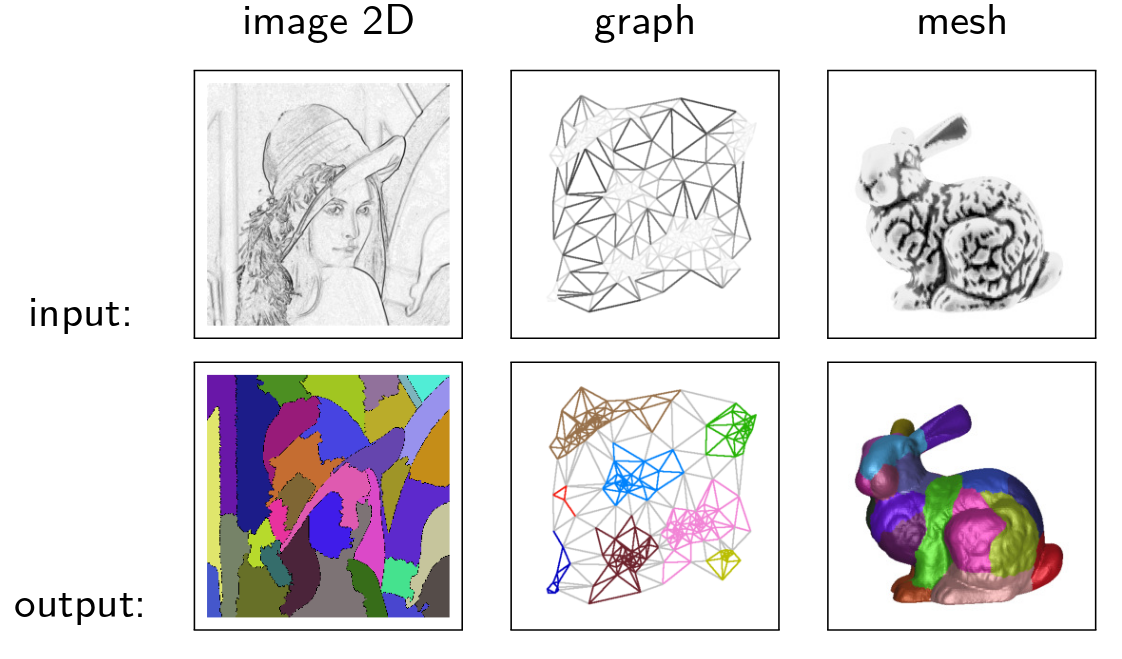
\includegraphics[height=5cm]{figs/type_vs_algo.png}
  \caption{Watershed algorithm applied to three different image types}
  \label{fig.type.vs.algo2}
\end{figure}

Tools able to handle many data representations are said to be \emph{generic}. In the particular case of a \emph{library}
providing a set of \emph{routines}, \emph{genericity} means that the \emph{routines} can be applied to a variety of
inputs (as opposed to \emph{specific} routines that support inputs of unique \emph{predefined} type). As an example,
consider the morphological \emph{dilation} that takes two inputs: an image and a flat structuring element (SE). Then,
the set of some possible inputs is depicted in~\cref{fig.espaceSAV}. Note that in this example, the image is already a
type product between the underlying \emph{structure kind} and the \emph{value kind}. Let $s$ be the number of
structures, $v$ the number of types of values, and $k$ the number of structuring elements. With no
\emph{generalization}, one would have to write $s \times v \times k$ \emph{dilation} routines.

\begin{figure}[htbp]
  \centering
  \subcaptionbox{}{\includestandalone[width=.48\linewidth]{figs/espaceSeI}}
  \subcaptionbox{}{\includestandalone[width=.48\linewidth]{figs/espaceSAV}}
  \caption{The space of possible implementation of the \emph{dilation(image, se)}
    routine. The image axis shown in (a) is in-fact multidimensional and should
    be considered 2D as in (b).}
  \label{fig.espaceSAV}
\end{figure}

Many IP libraries have emerged, developed in many programming languages. They all faced this problem and tried to bring
solutions, some of which are reviewed in \cref{part.motivations_and_context}. Among these solutions, we see that
\emph{generic programming} is good starting point~\cite{geraud.2000.icpr} to design a \emph{generic} library but still
has many problem. In particular, we focus on the case of \textsc{Milena}~\cite{levillain.2010.icip,
  geraud.2012.ipolmeeting}, a generic pre-modern C++ IP libray and its shortcomings that led to the design of
\textsc{Pylena}~\cite{carlinet.2018.pylena}.  The work presented in this paper contrasts with the previous works on
obtaining genericity for mathematical morphology operators~\cite{darbon.2002.ismm,levillain.2009.ismm} and digital
topology operators~\cite{levillain.2012.wadgmm-lncs}.

In \cref{part.genericity}, we present this new generic design, that emerged with the evolution of the Modern C++ and
allowed solving some \textsc{Milena}'s shortcomings. Not only does this new design re-conciliate \emph{simplicity} and
\emph{performance}, but it also promotes \emph{extensibility} as it enables easily creating custom image types as those
shown in \cref{part.image_views}.


\vspace{1cm}

Our work on bringing genericity to image processing through C++ template metaprogramming and concepts is presented
in~\citep{roynard.2019.rrpr}. Continuing this previous work, we focused on the main goals of the library. First is the
zero-cost of traversing an image, overhauling the existing system which is macro-based. The new system presented in
section~\ref{part.image_views} is based on
range-v3~\cite{niebler.2014.ranges,niebler.2018.deepranges,niebler.2018.mergingranges}. Following, we will show in
section~\ref{part.image_views} a design around image's domain definition, extension and structuring element: how those
concepts link with each other when used to write local algorithms. Another objective of the library is the ease of use
and the binding with existing ecosystem, such as Python and NumPy. So we will present in
section~\ref{part.static_dynamic_bridge} our work about binding a generic C++ library to python. Finally, we will
discuss in section~\ref{part.image_and_algorithms_taxonomy} the issue of heterogeneous computing. We offer an avenue
around the idea of canvas algorithm that can be exploited to bring performance without being intrusive for the user.
Though it comes with its lot of disadvantage, such as a paradigm switch to event-driven programming.
